PDTs \cite{Wei2022} are a type of decision tree model that incorporates probabilistic information into the decision-making process. Unlike traditional decision trees that make deterministic decisions based on fixed rules, PDTs assign probabilities to each possible outcome at each decision node. Considering a dataset of a set of features as inputs \emath{I} and a set of output features \emath{Q} that are used mainly for reasoning, we can define PDTs as follows: 



\begin{mydef} A PDT is represented as a tuple \emath{\mathcal{DT}=\langle I, G, X, Rule\rangle}, where:  
 \begin{itemize}
\item \emath{I}  represents a set of input features 
\item \emath{G} is a set of constraints applied over \emath{I}  and 
\item \emath{X} represents a set of feature values. We define \emath{g_{i}} as a constraint on each input feature \emath{I}  and \emath{eval_{v}: I \rightarrow \mathbb{D}} to evaluate the features of the PDT. Here, \emath{v_{0},\ldots,v_{n}} denote the valuations of the output features. 
 \end{itemize}
When exploring the tree from the root to the leaf, a rule takes the form of \emath{x_{0} \wedge \ldots \wedge x_{n} \rightarrow_{\lambda} x_{n+1}\wedge \ldots \wedge x_{n+j}}, where \emath{\lambda} represents the probability of occurrence of the rule in the dataset and  \emath{x_{0}\models g_{0} \ldots \wedge x_{n} \models g_{n}.}We use \emath{\sset{\mathcal{P}_\mathcal{DT}}} to identify a set of rules derived from the dataset.
\end{mydef}


The example in \fig{fig:pdt} shows the structure of the PDT, where each node represents an input feature \emath{I=\{\texttt{CO2}, \texttt{Humidity}\}}, except for the leaf node, which represents the output feature \emath{I= I \cup \{ \texttt{Ventilation} \}}. In this specific case, we can interpret the following rule: \texttt{CO2 >= High }$\wedge$ \texttt{humidity >= 80}\% $\rightarrow_{1}$ \texttt{Ventilation level= 2}
\noindent
\begin{figure}[!htb]
    \centering
    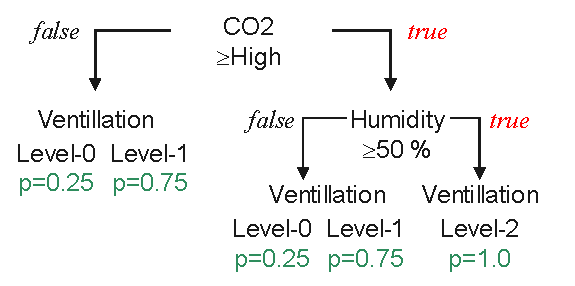
\includegraphics[width=150pt, height =82pt]{decisiontreeexample.pdf}
    \caption{Example of a PDT}
    \label{fig:pdt}
\end{figure} 

The formalism of \cmt{PDT} can be encompassed within the formalism of Probabilistic Automata (PA), where the states capture the PDT features and transition the evolution of state features.


% \begin{mydef} A PA of a Probabilistic Decision Tree is represented as a tuple \emath{\mathcal{DT}_{\mathcal{P}} =\langle  S_{0}, S, \Sigma, AP, L, \delta\rangle}, where:
% \label{ts}
% \begin{itemize}
% 	\item \emath{S_{0} = (\langle x_{0},\ldots,x_{n}, \theta \rangle )} is an initial state that corresponds to the initial variable values.
 
% 	\item \emath{S=\mathbb{D}^{I}} is the domain of \emath{\mathcal{DT}} features \emath{I},

% 	\item \emath{\Sigma}  is a finite set of decision rules label,

%     \item \emath{AP = S \cup G},

%  	\item \emath{L(\langle s,\theta\rangle ) = \{ s\} \cup \{ g \in G\} | \theta \models g}, and

%     \item \emath{\delta : S \times \Sigma \rightarrow Dist(S)} is a probabilistic transition function assigning for each \emath{s \in S} and \emath{\alpha \in \Sigma } a probabilistic distribution \emath{\mu \in Dist(S)} that are represented by the following operational semantics rules:

%    \begin{boxD}
   
%    \begin{equation}\frac{ s \gparrow{\tau} s' \ s\models g} { \langle s, \theta\rangle \xrightarrow{\tau}\langle s'_{0}, \theta' \rangle  } \label{eq1} \tag{ \emph{  Nom-probabilistic \emath{\mathcal{DT} rule}}} 
%    \end{equation}
%     where  \emath{\theta' =\theta[x'_{0}= eval(x_{0}) \wedge \ldots \wedge x'_{n}=eval(x_{n})]} 

%       \begin{equation}\frac{ s \gparrow{\tau}_{\lambda} s' \ s\models g} { \langle s, \theta\rangle \xrightarrow{\tau}_{\lambda}\langle s'_{0}, \theta' \rangle  } \label{eq1} \tag{ \emph{  Probabilistic \emath{\mathcal{DT} rule}}} 
%    \end{equation}
   
%      where  \emath{\theta' =\theta[x'_{0}= eval(x_{0}) \wedge \ldots \wedge x'_{n}=eval(x_{n})]} 
  
%   \end{boxD}
              
% \end{itemize}
% \end{mydef}
